\section{Solution}

``
Solution: describes your solution of the task.
Contains a detailed description of all the subtasks which have been solved and how they contribute to the solution for the given task.
The use of diagrams, figures, tables and similar is welcome as a support to your description.
``

% TODO: Putt dette i introduksjonen? Eventuelt putt lista i et vedlegg
\subsection{Development Process \& Tools}

Development was done on computers in the computer lab running Ubuntu 12.04.
In addition, we used Microsoft Remote Desktop to be able to use Xilinx from other locations.
ghdl and gtkwave also proved useful, as it allowed us to work locally when only writing and testing vhdl modules. Figure \ref{fig:software} lists all the software used.

\begin{figure}[ht!]
    \begin{description}
        \item{\textbf{ISE Project Navigator 12.4 M.81d}}
            Main IDE for writing and synthesizing VHDL.
        \item{\textbf{ISim 12.4 M.81d}}
            Simulation environment for simulating VHDL.
        \item{\textbf{hostcomm 1.0.0}}
            Programming utility for the Spartan-6 LX16 Evaluation Kit.
        \item{\textbf{VIM}}
            For text editing.
        \item{\textbf{GHDL}}
            Allowed for writing and testing components on Mac OS X.
        \item{\textbf{gtkwave}}
            Visualization tool for inspecting test simulations run with ghdl.
        \item{\textbf{git \& GitHub}}
            Version control system with central code repository hosting.
    \label{fig:software}
    \end{description}
    \caption{Software used during the development process}
\end{figure}

\subsection{Architecture}

The architecture is based on the drawing from the lecture slides 4 \cite{lecture-4}.
However because of the test environment and the lack of shift on immideate jump values,
the design was altered to suit our needs.
The final design is visible in the figure %\ref{fig:final-design} %TODO: skal vi ha fila her?

One big change is the external memory which is not present in the suggested architecture.
This difference made it so that the memory module is not needed.
Because all interaction is done with the external memory directly.
In changing the design the processor has gone from a von Neumann architecture to a full Hardvard architecture.
An advantage of this is the lack of a need to abstract away two separate external memories when no benfit is gained.

\subsubsection{MIPS subset}

The final processor design implements the following subset of the MIPS instruction set.

\begin{itemize}
    \item ALU instructions (ADD, SUB, SLT, AND, OR, SLL, SRL)
    \item Conditional Branch (BEZ)
    \item Jump Instruction (JMP)
    \item LOAD, STORE, Load immediate (LW, SW, LDI)
\end{itemize}

Note: the {\bf LDI} (Load Immediate) instruction is not a part of the MIPS instruction set\footnote{Figure C.1 \cite[p.66]{compendium}}.
The {\bf LUI} (Load Upper Immediate) is the closest match.
This instruction loads the value into the upper 16 bits of the register.
The support files handed out already used this instruction.

\subsubsection{State machine}

The control unit is based on the state machine from lecture 4. \cite{lecture-4}
It has been modified to add support for the extra load upper immediate instruction.
Output signals which were not needed in our architecture are also removed.
Specifically, the i\_or\_d and mem\_read signals were not needed, because our processor has separate instruction and data memories.
Because of the latency when reading from memory the ir\_write signal has been moved to the instruction\_decode state, when the correct instruction has been fetched.
This does not cause any latency issues, as the instruction register is designed to let the new instruction value through when ir\_write is high.
A state diagram for the control unit can be seen in figure \ref{fig:state_machine}.

\begin{figure}[ht!]
    \begin{center}
    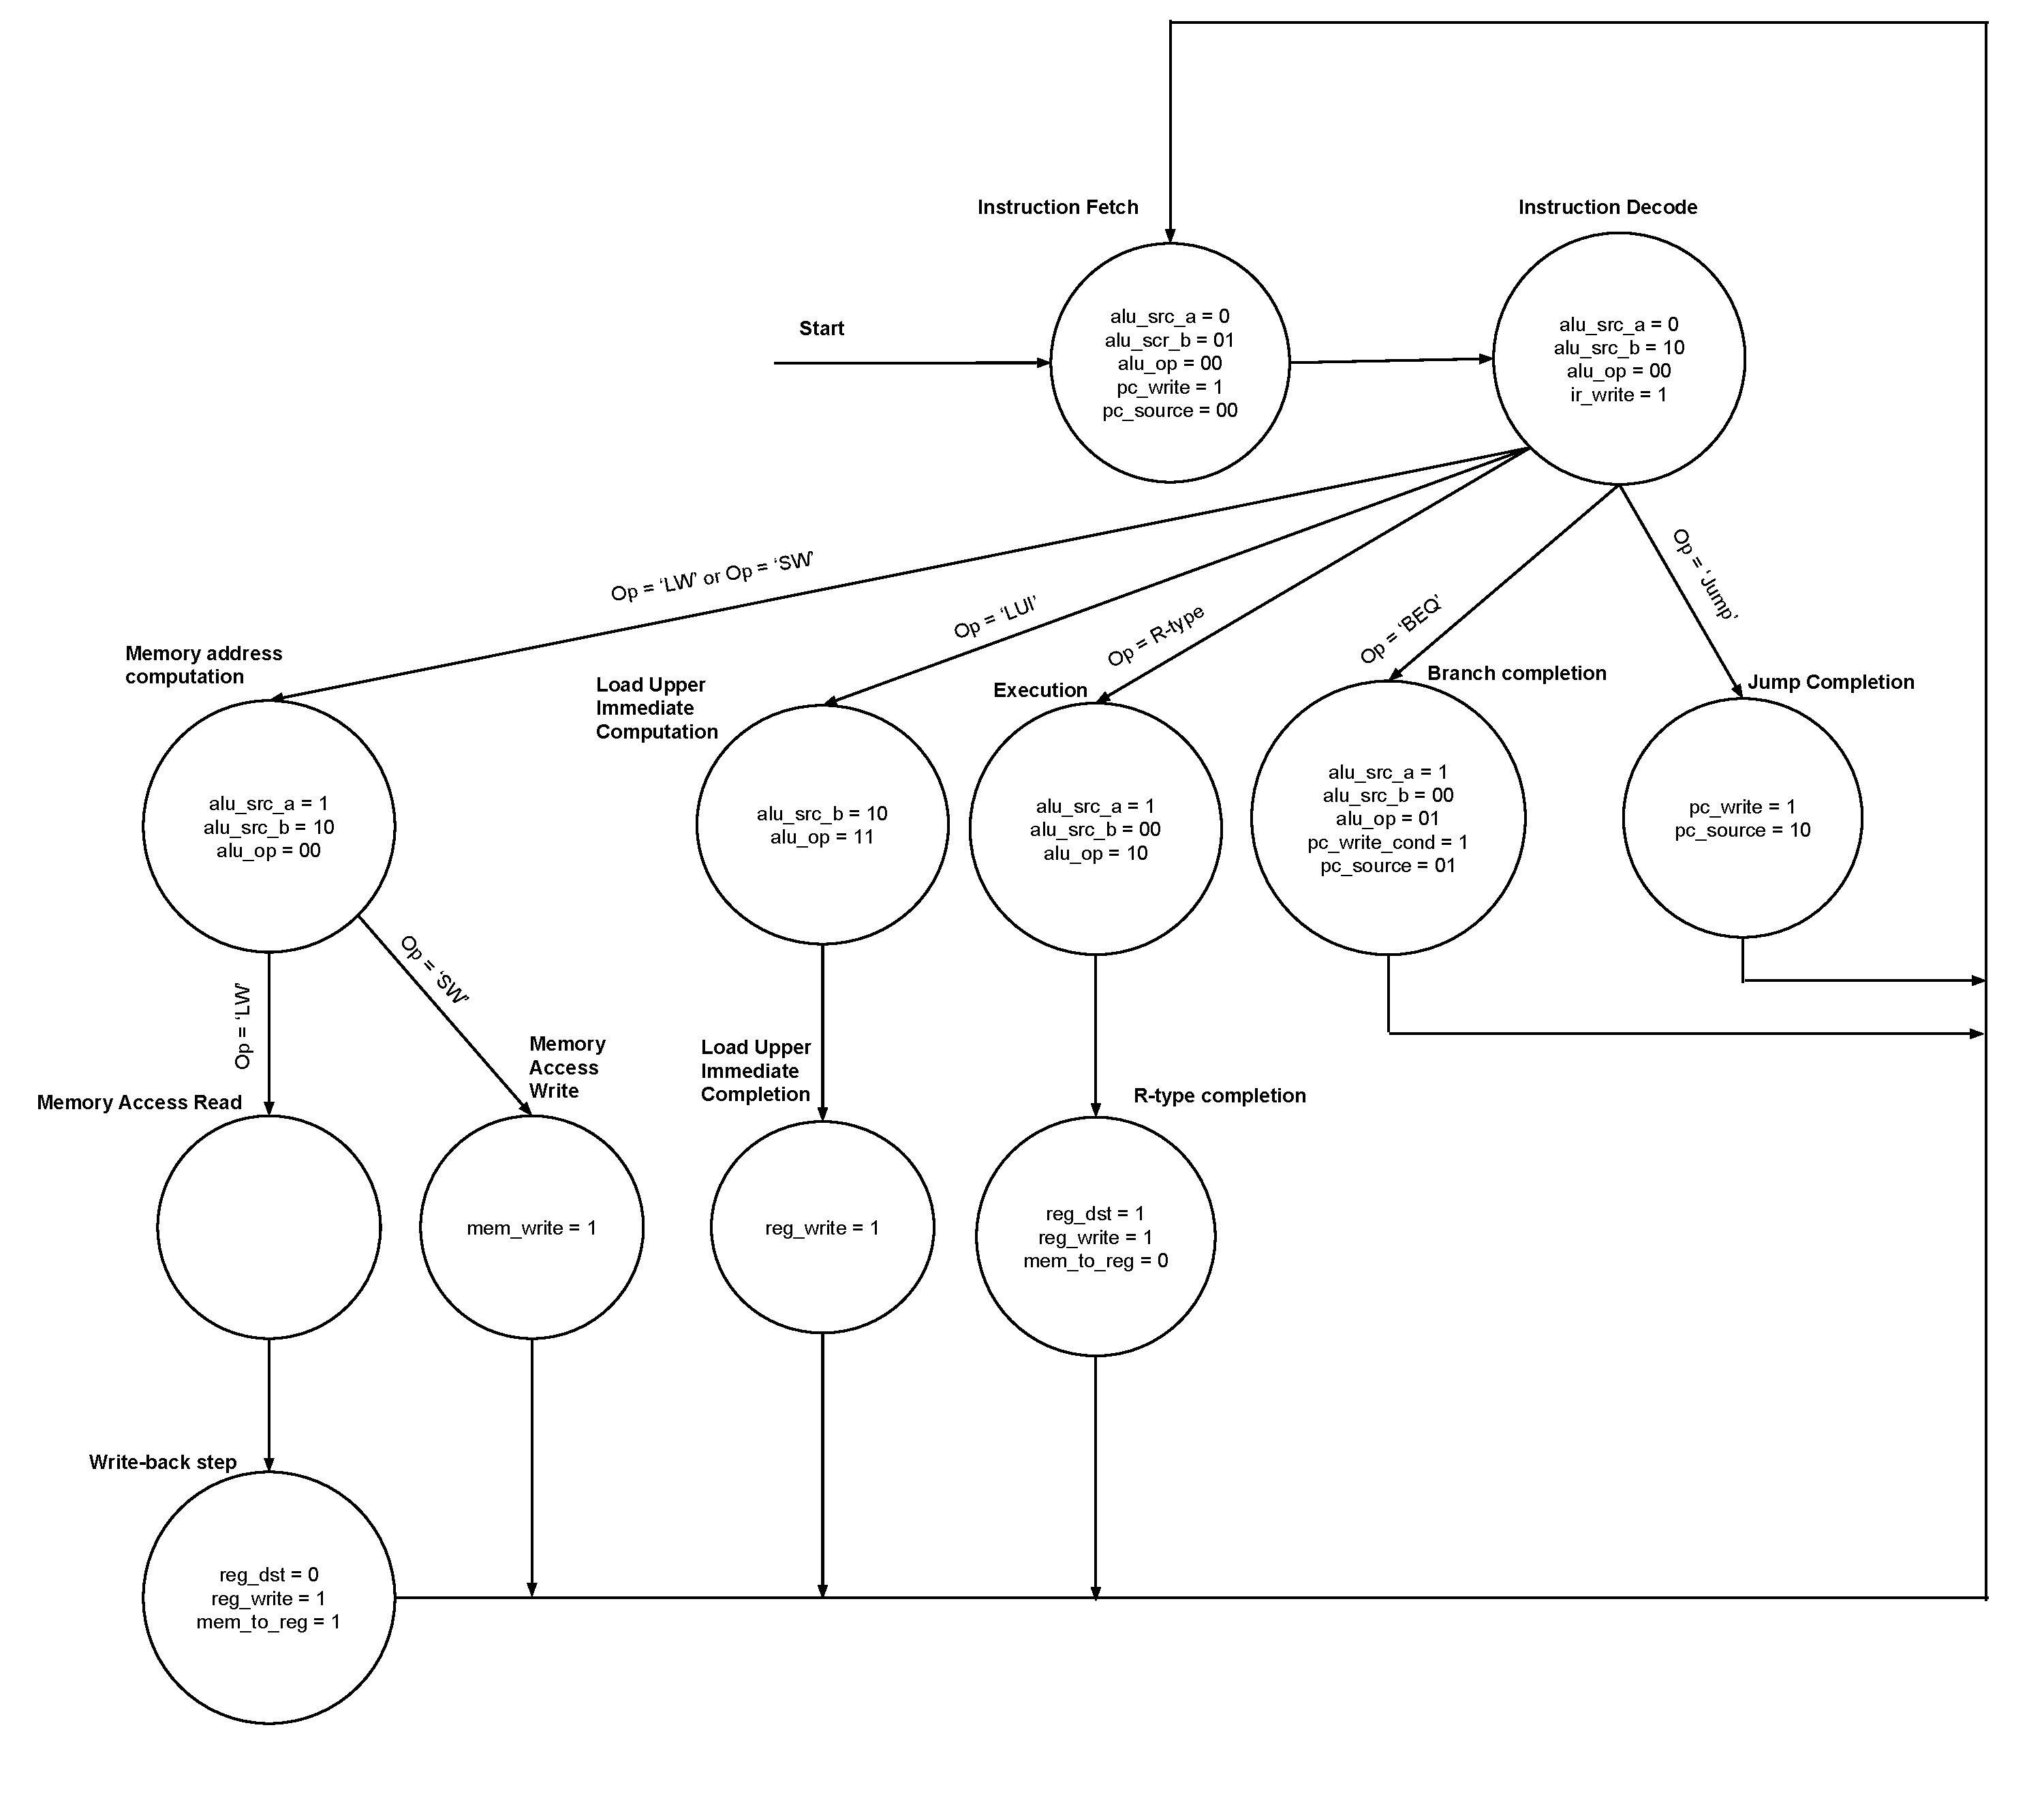
\includegraphics[width=\textwidth]{assets/state_machine.pdf}
    \caption{State diagram for the control unit}
    \label{fig:state_machine}
    \end{center}
\end{figure}

\subsubsection{RTL schematic}

\subsection{Implementation}

\subsubsection{Modularization}

\begin{table}
    \begin{tabular}{|l|l|l|l|l|l|l|}
    \hline
    Opcode & ALUOp & Operation           & Function & ALU Function        & ALU Control & Shamt   \\ \hline
    lw     & 00    & load word           & XXXXXX   & add                 & ADD         & \\ \hline
    sw     & 00    & store word          & XXXXXX   & add                 & ADD         & \\ \hline
    beq    & 01    & branch equal        & XXXXXX   & subtract            & SUBTRACT    & \\ \hline
    r-type & 10    & add                 & 100000   & add                 & ADD         & \\ \cline{3-7}
           &       & subtract            & 100010   & subtract            & SUBTRACT    & \\ \cline{3-7}
           &       & AND                 & 100100   & AND                 & AND         & \\ \cline{3-7}
           &       & OR                  & 100101   & OR                  & OR          & \\ \cline{3-7}
           &       & set-on-less-than    & 101010   & set-on-less-than    & SLT         & \\ \cline{3-7}
           &       & shift-left-logical  & 000000   & shift-left-logical  & SLL         & \\ \cline{3-7}
           &       & shift-right-logical & 000010   & shift-right-logical & SRL         & \\ \hline
    lui    & 11    & lui                 & XXXXXX   & add                 & ADD         & 10000 \\ \hline
    \end{tabular}
\end{table}

Bottom-up approach, unit tests, integration tests

\subsection{Optimizing for FPGA}


Things to write about

\begin{enumerate}
  \item
    Chip select on ram, power savings

  \item
    The war on Xilinx ISE. Learning experiences etschetera

  \item
    Block ram in Registers instead of flip-flops with gigantic muxes. The reason for this is that a hardware designer has to consider his platform, in this case the target was an FPGA, and not 'actual' hardware. FPGAs hate muxes , altho they might be better in real hardware. like -- insert explicitive here --. Mention the LUT savings here. Like 2445 to 750 luts!!!! wow such save.

  \item
    State machine is based on the multicycle mips architecture provided in lecture slides.

  \item
    Outsourcing ALU control values to vhdl ENUM as it is better than us to assign logic values!

  \item
    Reducing critical path to increase clock frequency. Worst path is instruction immediate -> alu latch B -> alu -> zero out -> PC write.


\end{enumerate}
